\documentclass[1p]{elsarticle_modified}
%\bibliographystyle{elsarticle-num}

%\usepackage[colorlinks]{hyperref}
%\usepackage{abbrmath_seonhwa} %\Abb, \Ascr, \Acal ,\Abf, \Afrak
\usepackage{amsfonts}
\usepackage{amssymb}
\usepackage{amsmath}
\usepackage{amsthm}
\usepackage{scalefnt}
\usepackage{amsbsy}
\usepackage{kotex}
\usepackage{caption}
\usepackage{subfig}
\usepackage{color}
\usepackage{graphicx}
\usepackage{xcolor} %% white, black, red, green, blue, cyan, magenta, yellow
\usepackage{float}
\usepackage{setspace}
\usepackage{hyperref}

\usepackage{tikz}
\usetikzlibrary{arrows}

\usepackage{multirow}
\usepackage{array} % fixed length table
\usepackage{hhline}

%%%%%%%%%%%%%%%%%%%%%
\makeatletter
\renewcommand*\env@matrix[1][\arraystretch]{%
	\edef\arraystretch{#1}%
	\hskip -\arraycolsep
	\let\@ifnextchar\new@ifnextchar
	\array{*\c@MaxMatrixCols c}}
\makeatother %https://tex.stackexchange.com/questions/14071/how-can-i-increase-the-line-spacing-in-a-matrix
%%%%%%%%%%%%%%%

\usepackage[normalem]{ulem}

\newcommand{\msout}[1]{\ifmmode\text{\sout{\ensuremath{#1}}}\else\sout{#1}\fi}
%SOURCE: \msout is \stkout macro in https://tex.stackexchange.com/questions/20609/strikeout-in-math-mode

\newcommand{\cancel}[1]{
	\ifmmode
	{\color{red}\msout{#1}}
	\else
	{\color{red}\sout{#1}}
	\fi
}

\newcommand{\add}[1]{
	{\color{blue}\uwave{#1}}
}

\newcommand{\replace}[2]{
	\ifmmode
	{\color{red}\msout{#1}}{\color{blue}\uwave{#2}}
	\else
	{\color{red}\sout{#1}}{\color{blue}\uwave{#2}}
	\fi
}

\newcommand{\Sol}{\mathcal{S}} %segment
\newcommand{\D}{D} %diagram
\newcommand{\A}{\mathcal{A}} %arc


%%%%%%%%%%%%%%%%%%%%%%%%%%%%%5 test

\def\sl{\operatorname{\textup{SL}}(2,\Cbb)}
\def\psl{\operatorname{\textup{PSL}}(2,\Cbb)}
\def\quan{\mkern 1mu \triangleright \mkern 1mu}

\theoremstyle{definition}
\newtheorem{thm}{Theorem}[section]
\newtheorem{prop}[thm]{Proposition}
\newtheorem{lem}[thm]{Lemma}
\newtheorem{ques}[thm]{Question}
\newtheorem{cor}[thm]{Corollary}
\newtheorem{defn}[thm]{Definition}
\newtheorem{exam}[thm]{Example}
\newtheorem{rmk}[thm]{Remark}
\newtheorem{alg}[thm]{Algorithm}

\newcommand{\I}{\sqrt{-1}}
\begin{document}

%\begin{frontmatter}
%
%\title{Boundary parabolic representations of knots up to 8 crossings}
%
%%% Group authors per affiliation:
%\author{Yunhi Cho} 
%\address{Department of Mathematics, University of Seoul, Seoul, Korea}
%\ead{yhcho@uos.ac.kr}
%
%
%\author{Seonhwa Kim} %\fnref{s_kim}}
%\address{Center for Geometry and Physics, Institute for Basic Science, Pohang, 37673, Korea}
%\ead{ryeona17@ibs.re.kr}
%
%\author{Hyuk Kim}
%\address{Department of Mathematical Sciences, Seoul National University, Seoul 08826, Korea}
%\ead{hyukkim@snu.ac.kr}
%
%\author{Seokbeom Yoon}
%\address{Department of Mathematical Sciences, Seoul National University, Seoul, 08826,  Korea}
%\ead{sbyoon15@snu.ac.kr}
%
%\begin{abstract}
%We find all boundary parabolic representation of knots up to 8 crossings.
%
%\end{abstract}
%\begin{keyword}
%    \MSC[2010] 57M25 
%\end{keyword}
%
%\end{frontmatter}

%\linenumbers
%\tableofcontents
%
\newcommand\colored[1]{\textcolor{white}{\rule[-0.35ex]{0.8em}{1.4ex}}\kern-0.8em\color{red} #1}%
%\newcommand\colored[1]{\textcolor{white}{ #1}\kern-2.17ex	\textcolor{white}{ #1}\kern-1.81ex	\textcolor{white}{ #1}\kern-2.15ex\color{red}#1	}

{\Large $\underline{12a_{0367}~(K12a_{0367})}$}

\setlength{\tabcolsep}{10pt}
\renewcommand{\arraystretch}{1.6}
\vspace{1cm}\begin{tabular}{m{100pt}>{\centering\arraybackslash}m{274pt}}
\multirow{5}{120pt}{
	\centering
	\includegraphics[width=112pt]{../../../GIT/diagram.site/Diagrams/png/1168_12a_0367.png}\\
\ \ \ A knot diagram\footnotemark}&
\allowdisplaybreaks
\textbf{Linearized knot diagam} \\
\cline{2-2}
 &
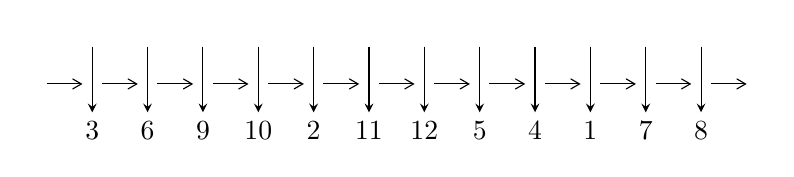
\begin{tikzpicture}[x=20pt, y=17pt]
	% nodes
	\node (C0) at (0, 0) {};
	\node (C1) at (1, 0) {};
	\node (C1U) at (1, +1) {};
	\node (C1D) at (1, -1) {3};

	\node (C2) at (2, 0) {};
	\node (C2U) at (2, +1) {};
	\node (C2D) at (2, -1) {6};

	\node (C3) at (3, 0) {};
	\node (C3U) at (3, +1) {};
	\node (C3D) at (3, -1) {9};

	\node (C4) at (4, 0) {};
	\node (C4U) at (4, +1) {};
	\node (C4D) at (4, -1) {10};

	\node (C5) at (5, 0) {};
	\node (C5U) at (5, +1) {};
	\node (C5D) at (5, -1) {2};

	\node (C6) at (6, 0) {};
	\node (C6U) at (6, +1) {};
	\node (C6D) at (6, -1) {11};

	\node (C7) at (7, 0) {};
	\node (C7U) at (7, +1) {};
	\node (C7D) at (7, -1) {12};

	\node (C8) at (8, 0) {};
	\node (C8U) at (8, +1) {};
	\node (C8D) at (8, -1) {5};

	\node (C9) at (9, 0) {};
	\node (C9U) at (9, +1) {};
	\node (C9D) at (9, -1) {4};

	\node (C10) at (10, 0) {};
	\node (C10U) at (10, +1) {};
	\node (C10D) at (10, -1) {1};

	\node (C11) at (11, 0) {};
	\node (C11U) at (11, +1) {};
	\node (C11D) at (11, -1) {7};

	\node (C12) at (12, 0) {};
	\node (C12U) at (12, +1) {};
	\node (C12D) at (12, -1) {8};
	\node (C13) at (13, 0) {};

	% arrows
	\draw[->,>={angle 60}]
	(C0) edge (C1) (C1) edge (C2) (C2) edge (C3) (C3) edge (C4) (C4) edge (C5) (C5) edge (C6) (C6) edge (C7) (C7) edge (C8) (C8) edge (C9) (C9) edge (C10) (C10) edge (C11) (C11) edge (C12) (C12) edge (C13) ;	\draw[->,>=stealth]
	(C1U) edge (C1D) (C2U) edge (C2D) (C3U) edge (C3D) (C4U) edge (C4D) (C5U) edge (C5D) (C6U) edge (C6D) (C7U) edge (C7D) (C8U) edge (C8D) (C9U) edge (C9D) (C10U) edge (C10D) (C11U) edge (C11D) (C12U) edge (C12D) ;
	\end{tikzpicture} \\
\hhline{~~} \\& 
\textbf{Solving Sequence} \\ \cline{2-2} 
 &
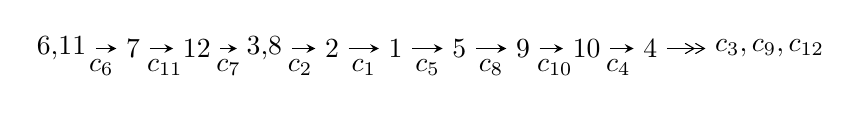
\begin{tikzpicture}[x=23pt, y=7pt]
	% node
	\node (A0) at (-1/8, 0) {6,11};
	\node (A1) at (1, 0) {7};
	\node (A2) at (2, 0) {12};
	\node (A3) at (49/16, 0) {3,8};
	\node (A4) at (33/8, 0) {2};
	\node (A5) at (41/8, 0) {1};
	\node (A6) at (49/8, 0) {5};
	\node (A7) at (57/8, 0) {9};
	\node (A8) at (65/8, 0) {10};
	\node (A9) at (73/8, 0) {4};
	\node (C1) at (1/2, -1) {$c_{6}$};
	\node (C2) at (3/2, -1) {$c_{11}$};
	\node (C3) at (5/2, -1) {$c_{7}$};
	\node (C4) at (29/8, -1) {$c_{2}$};
	\node (C5) at (37/8, -1) {$c_{1}$};
	\node (C6) at (45/8, -1) {$c_{5}$};
	\node (C7) at (53/8, -1) {$c_{8}$};
	\node (C8) at (61/8, -1) {$c_{10}$};
	\node (C9) at (69/8, -1) {$c_{4}$};
	\node (A10) at (11, 0) {$c_{3},c_{9},c_{12}$};

	% edge
	\draw[->,>=stealth]	
	(A0) edge (A1) (A1) edge (A2) (A2) edge (A3) (A3) edge (A4) (A4) edge (A5) (A5) edge (A6) (A6) edge (A7) (A7) edge (A8) (A8) edge (A9) ;
	\draw[->>,>={angle 60}]	
	(A9) edge (A10);
\end{tikzpicture} \\ 

\end{tabular} \\

\footnotetext{
The image of knot diagram is generated by the software ``\textbf{Draw programme}" developed by Andrew Bartholomew(\url{http://www.layer8.co.uk/maths/draw/index.htm\#Running-draw}), where we modified some parts for our purpose(\url{https://github.com/CATsTAILs/LinksPainter}).
}\phantom \\ \newline 
\centering \textbf{Ideals for irreducible components\footnotemark of $X_{\text{par}}$} 
 
\begin{align*}
I^u_{1}&=\langle 
-5.26039\times10^{20} u^{71}-3.31809\times10^{22} u^{70}+\cdots+4.33870\times10^{22} b+1.79186\times10^{22},\\
\phantom{I^u_{1}}&\phantom{= \langle  }-8.36919\times10^{22} u^{71}+1.25008\times10^{23} u^{70}+\cdots+8.67739\times10^{22} a+3.24699\times10^{22},\;u^{72}-2 u^{71}+\cdots+2 u+1\rangle \\
I^u_{2}&=\langle 
b-1,\;a^2-2 a+2 u-3,\;u^2- u-1\rangle \\
I^u_{3}&=\langle 
b+1,\;a+1,\;u^2+u-1\rangle \\
\\
\end{align*}
\raggedright * 3 irreducible components of $\dim_{\mathbb{C}}=0$, with total 78 representations.\\
\footnotetext{All coefficients of polynomials are rational numbers. But the coefficients are sometimes approximated in decimal forms when there is not enough margin.}
\newpage
\renewcommand{\arraystretch}{1}
\centering \section*{I. $I^u_{1}= \langle -5.26\times10^{20} u^{71}-3.32\times10^{22} u^{70}+\cdots+4.34\times10^{22} b+1.79\times10^{22},\;-8.37\times10^{22} u^{71}+1.25\times10^{23} u^{70}+\cdots+8.68\times10^{22} a+3.25\times10^{22},\;u^{72}-2 u^{71}+\cdots+2 u+1 \rangle$}
\flushleft \textbf{(i) Arc colorings}\\
\begin{tabular}{m{7pt} m{180pt} m{7pt} m{180pt} }
\flushright $a_{6}=$&$\begin{pmatrix}1\\0\end{pmatrix}$ \\
\flushright $a_{11}=$&$\begin{pmatrix}0\\u\end{pmatrix}$ \\
\flushright $a_{7}=$&$\begin{pmatrix}1\\u^2\end{pmatrix}$ \\
\flushright $a_{12}=$&$\begin{pmatrix}- u\\- u^3+u\end{pmatrix}$ \\
\flushright $a_{3}=$&$\begin{pmatrix}0.964482 u^{71}-1.44061 u^{70}+\cdots-11.9876 u-0.374190\\0.0121244 u^{71}+0.764766 u^{70}+\cdots+0.453521 u-0.412996\end{pmatrix}$ \\
\flushright $a_{8}=$&$\begin{pmatrix}- u^2+1\\- u^4+2 u^2\end{pmatrix}$ \\
\flushright $a_{2}=$&$\begin{pmatrix}0.976607 u^{71}-0.675847 u^{70}+\cdots-11.5341 u-0.787186\\0.0121244 u^{71}+0.764766 u^{70}+\cdots+0.453521 u-0.412996\end{pmatrix}$ \\
\flushright $a_{1}=$&$\begin{pmatrix}u^3-2 u\\u^5-3 u^3+u\end{pmatrix}$ \\
\flushright $a_{5}=$&$\begin{pmatrix}-1.98741 u^{71}+1.11158 u^{70}+\cdots+14.3859 u+3.65867\\-0.926705 u^{71}+0.404836 u^{70}+\cdots+1.82730 u+0.532714\end{pmatrix}$ \\
\flushright $a_{9}=$&$\begin{pmatrix}0.472718 u^{71}-1.08136 u^{70}+\cdots-16.3593 u-1.33874\\-1.10315 u^{71}+1.20031 u^{70}+\cdots+2.20486 u+0.947164\end{pmatrix}$ \\
\flushright $a_{10}=$&$\begin{pmatrix}u^7-4 u^5+4 u^3\\u^9-5 u^7+7 u^5-2 u^3+u\end{pmatrix}$ \\
\flushright $a_{4}=$&$\begin{pmatrix}-1.55989 u^{71}+0.727017 u^{70}+\cdots+13.9611 u+3.63430\\-0.566397 u^{71}+0.322301 u^{70}+\cdots-0.405449 u-0.412002\end{pmatrix}$\\&\end{tabular}
\flushleft \textbf{(ii) Obstruction class $= -1$}\\~\\
\flushleft \textbf{(iii) Cusp Shapes $= -\frac{124925391140869705539849}{43386961394563898337977} u^{71}+\frac{155786602228314171185371}{43386961394563898337977} u^{70}+\cdots+\frac{536149016094843518284893}{43386961394563898337977} u-\frac{597134730501655502761745}{43386961394563898337977}$}\\~\\
\newpage\renewcommand{\arraystretch}{1}
\flushleft \textbf{(iv) u-Polynomials at the component}\newline \\
\begin{tabular}{m{50pt}|m{274pt}}
Crossings & \hspace{64pt}u-Polynomials at each crossing \\
\hline $$\begin{aligned}c_{1}\end{aligned}$$&$\begin{aligned}
&u^{72}+37 u^{71}+\cdots+29 u+1
\end{aligned}$\\
\hline $$\begin{aligned}c_{2},c_{5}\end{aligned}$$&$\begin{aligned}
&u^{72}+3 u^{71}+\cdots+7 u+1
\end{aligned}$\\
\hline $$\begin{aligned}c_{3},c_{4},c_{9}\end{aligned}$$&$\begin{aligned}
&u^{72}- u^{71}+\cdots-12 u-4
\end{aligned}$\\
\hline $$\begin{aligned}c_{6},c_{7},c_{11}\\c_{12}\end{aligned}$$&$\begin{aligned}
&u^{72}-2 u^{71}+\cdots+2 u+1
\end{aligned}$\\
\hline $$\begin{aligned}c_{8}\end{aligned}$$&$\begin{aligned}
&u^{72}+3 u^{71}+\cdots+1492 u+220
\end{aligned}$\\
\hline $$\begin{aligned}c_{10}\end{aligned}$$&$\begin{aligned}
&u^{72}-20 u^{71}+\cdots-348 u+113
\end{aligned}$\\
\hline
\end{tabular}\\~\\
\newpage\renewcommand{\arraystretch}{1}
\flushleft \textbf{(v) Riley Polynomials at the component}\newline \\
\begin{tabular}{m{50pt}|m{274pt}}
Crossings & \hspace{64pt}Riley Polynomials at each crossing \\
\hline $$\begin{aligned}c_{1}\end{aligned}$$&$\begin{aligned}
&y^{72}+3 y^{71}+\cdots-197 y+1
\end{aligned}$\\
\hline $$\begin{aligned}c_{2},c_{5}\end{aligned}$$&$\begin{aligned}
&y^{72}-37 y^{71}+\cdots-29 y+1
\end{aligned}$\\
\hline $$\begin{aligned}c_{3},c_{4},c_{9}\end{aligned}$$&$\begin{aligned}
&y^{72}-67 y^{71}+\cdots-16 y+16
\end{aligned}$\\
\hline $$\begin{aligned}c_{6},c_{7},c_{11}\\c_{12}\end{aligned}$$&$\begin{aligned}
&y^{72}-84 y^{71}+\cdots-20 y+1
\end{aligned}$\\
\hline $$\begin{aligned}c_{8}\end{aligned}$$&$\begin{aligned}
&y^{72}-7 y^{71}+\cdots-402704 y+48400
\end{aligned}$\\
\hline $$\begin{aligned}c_{10}\end{aligned}$$&$\begin{aligned}
&y^{72}-12 y^{71}+\cdots-272524 y+12769
\end{aligned}$\\
\hline
\end{tabular}\\~\\
\newpage\flushleft \textbf{(vi) Complex Volumes and Cusp Shapes}
$$\begin{array}{c|c|c}  
\text{Solutions to }I^u_{1}& \I (\text{vol} + \sqrt{-1}CS) & \text{Cusp shape}\\
 \hline 
\begin{aligned}
u &= \phantom{-}0.928218 + 0.309234 I \\
a &= -0.354302 + 0.192132 I \\
b &= -1.065700 + 0.515640 I\end{aligned}
 & -7.24752 + 4.65448 I & \phantom{-0.000000 } 0 \\ \hline\begin{aligned}
u &= \phantom{-}0.928218 - 0.309234 I \\
a &= -0.354302 - 0.192132 I \\
b &= -1.065700 - 0.515640 I\end{aligned}
 & -7.24752 - 4.65448 I & \phantom{-0.000000 } 0 \\ \hline\begin{aligned}
u &= -0.737630 + 0.531689 I \\
a &= -0.70377 - 2.08141 I \\
b &= -1.166590 + 0.587970 I\end{aligned}
 & -5.52989 + 11.86830 I & \phantom{-0.000000 } 0 \\ \hline\begin{aligned}
u &= -0.737630 - 0.531689 I \\
a &= -0.70377 + 2.08141 I \\
b &= -1.166590 - 0.587970 I\end{aligned}
 & -5.52989 - 11.86830 I & \phantom{-0.000000 } 0 \\ \hline\begin{aligned}
u &= -0.884804 + 0.189140 I \\
a &= \phantom{-}0.504034 + 0.110912 I \\
b &= \phantom{-}0.931780 + 0.416732 I\end{aligned}
 & -2.20323 - 1.64389 I & \phantom{-0.000000 } 0 \\ \hline\begin{aligned}
u &= -0.884804 - 0.189140 I \\
a &= \phantom{-}0.504034 - 0.110912 I \\
b &= \phantom{-}0.931780 - 0.416732 I\end{aligned}
 & -2.20323 + 1.64389 I & \phantom{-0.000000 } 0 \\ \hline\begin{aligned}
u &= \phantom{-}0.883338 + 0.137471 I \\
a &= -0.750844 + 0.235422 I \\
b &= -0.381393 - 0.511313 I\end{aligned}
 & -5.31297 + 0.37168 I & -12.00000 + 0. I\phantom{ +0.000000I} \\ \hline\begin{aligned}
u &= \phantom{-}0.883338 - 0.137471 I \\
a &= -0.750844 - 0.235422 I \\
b &= -0.381393 + 0.511313 I\end{aligned}
 & -5.31297 - 0.37168 I & -12.00000 + 0. I\phantom{ +0.000000I} \\ \hline\begin{aligned}
u &= \phantom{-}0.690814 + 0.522826 I \\
a &= \phantom{-}0.56315 - 2.15893 I \\
b &= \phantom{-}1.099150 + 0.589092 I\end{aligned}
 & \phantom{-}0.02673 - 8.09347 I & -12.0000 + 9.2851 I \\ \hline\begin{aligned}
u &= \phantom{-}0.690814 - 0.522826 I \\
a &= \phantom{-}0.56315 + 2.15893 I \\
b &= \phantom{-}1.099150 - 0.589092 I\end{aligned}
 & \phantom{-}0.02673 + 8.09347 I & -12.0000 - 9.2851 I\\
 \hline 
 \end{array}$$\newpage$$\begin{array}{c|c|c}  
\text{Solutions to }I^u_{1}& \I (\text{vol} + \sqrt{-1}CS) & \text{Cusp shape}\\
 \hline 
\begin{aligned}
u &= -0.678297 + 0.515178 I \\
a &= \phantom{-}0.977292 + 0.542744 I \\
b &= -0.295256 - 0.854652 I\end{aligned}
 & -2.93335 + 6.55153 I & -14.6691 - 6.1676 I \\ \hline\begin{aligned}
u &= -0.678297 - 0.515178 I \\
a &= \phantom{-}0.977292 - 0.542744 I \\
b &= -0.295256 + 0.854652 I\end{aligned}
 & -2.93335 - 6.55153 I & -14.6691 + 6.1676 I \\ \hline\begin{aligned}
u &= -0.630548 + 0.470751 I \\
a &= -0.34238 - 2.38082 I \\
b &= -1.003340 + 0.528804 I\end{aligned}
 & -1.31023 + 3.89736 I & -15.2781 - 4.8812 I \\ \hline\begin{aligned}
u &= -0.630548 - 0.470751 I \\
a &= -0.34238 + 2.38082 I \\
b &= -1.003340 - 0.528804 I\end{aligned}
 & -1.31023 - 3.89736 I & -15.2781 + 4.8812 I \\ \hline\begin{aligned}
u &= -0.669262 + 0.404635 I \\
a &= \phantom{-}0.465808 + 0.565250 I \\
b &= \phantom{-}1.254740 + 0.247917 I\end{aligned}
 & -7.95058 + 3.07874 I & -19.9096 - 5.4080 I \\ \hline\begin{aligned}
u &= -0.669262 - 0.404635 I \\
a &= \phantom{-}0.465808 - 0.565250 I \\
b &= \phantom{-}1.254740 - 0.247917 I\end{aligned}
 & -7.95058 - 3.07874 I & -19.9096 + 5.4080 I \\ \hline\begin{aligned}
u &= \phantom{-}0.597312 + 0.499582 I \\
a &= -1.048900 + 0.571843 I \\
b &= \phantom{-}0.401917 - 0.758054 I\end{aligned}
 & \phantom{-}2.07881 - 2.99552 I & -9.38208 + 5.15386 I \\ \hline\begin{aligned}
u &= \phantom{-}0.597312 - 0.499582 I \\
a &= -1.048900 - 0.571843 I \\
b &= \phantom{-}0.401917 + 0.758054 I\end{aligned}
 & \phantom{-}2.07881 + 2.99552 I & -9.38208 - 5.15386 I \\ \hline\begin{aligned}
u &= \phantom{-}0.670676 + 0.356136 I \\
a &= \phantom{-}0.63994 - 3.06673 I \\
b &= \phantom{-}1.042790 + 0.370481 I\end{aligned}
 & -8.27974 - 2.07809 I & -20.0885 + 6.6662 I \\ \hline\begin{aligned}
u &= \phantom{-}0.670676 - 0.356136 I \\
a &= \phantom{-}0.63994 + 3.06673 I \\
b &= \phantom{-}1.042790 - 0.370481 I\end{aligned}
 & -8.27974 + 2.07809 I & -20.0885 - 6.6662 I\\
 \hline 
 \end{array}$$\newpage$$\begin{array}{c|c|c}  
\text{Solutions to }I^u_{1}& \I (\text{vol} + \sqrt{-1}CS) & \text{Cusp shape}\\
 \hline 
\begin{aligned}
u &= -0.464343 + 0.536069 I \\
a &= \phantom{-}0.09506 - 1.92402 I \\
b &= -0.761545 + 0.651812 I\end{aligned}
 & -0.22536 + 4.12491 I & -12.4469 - 7.3915 I \\ \hline\begin{aligned}
u &= -0.464343 - 0.536069 I \\
a &= \phantom{-}0.09506 + 1.92402 I \\
b &= -0.761545 - 0.651812 I\end{aligned}
 & -0.22536 - 4.12491 I & -12.4469 + 7.3915 I \\ \hline\begin{aligned}
u &= -0.154574 + 0.651894 I \\
a &= \phantom{-}0.81766 + 1.18825 I \\
b &= -1.116310 - 0.581761 I\end{aligned}
 & -3.80714 - 7.87957 I & -14.4786 + 4.9899 I \\ \hline\begin{aligned}
u &= -0.154574 - 0.651894 I \\
a &= \phantom{-}0.81766 - 1.18825 I \\
b &= -1.116310 + 0.581761 I\end{aligned}
 & -3.80714 + 7.87957 I & -14.4786 - 4.9899 I \\ \hline\begin{aligned}
u &= \phantom{-}0.614548 + 0.255524 I \\
a &= -0.757214 + 0.499889 I \\
b &= -1.130020 + 0.157751 I\end{aligned}
 & -2.78857 - 0.70974 I & -15.3214 + 8.6751 I \\ \hline\begin{aligned}
u &= \phantom{-}0.614548 - 0.255524 I \\
a &= -0.757214 - 0.499889 I \\
b &= -1.130020 - 0.157751 I\end{aligned}
 & -2.78857 + 0.70974 I & -15.3214 - 8.6751 I \\ \hline\begin{aligned}
u &= -0.432857 + 0.495289 I \\
a &= \phantom{-}1.20679 + 0.74677 I \\
b &= -0.640326 - 0.609624 I\end{aligned}
 & -0.159008 - 0.526549 I & -12.09743 - 0.07898 I \\ \hline\begin{aligned}
u &= -0.432857 - 0.495289 I \\
a &= \phantom{-}1.20679 - 0.74677 I \\
b &= -0.640326 + 0.609624 I\end{aligned}
 & -0.159008 + 0.526549 I & -12.09743 + 0.07898 I \\ \hline\begin{aligned}
u &= \phantom{-}0.207458 + 0.606070 I \\
a &= -0.95467 + 1.17138 I \\
b &= \phantom{-}1.020010 - 0.576008 I\end{aligned}
 & \phantom{-}1.44186 + 4.25219 I & -9.65797 - 4.16216 I \\ \hline\begin{aligned}
u &= \phantom{-}0.207458 - 0.606070 I \\
a &= -0.95467 - 1.17138 I \\
b &= \phantom{-}1.020010 + 0.576008 I\end{aligned}
 & \phantom{-}1.44186 - 4.25219 I & -9.65797 + 4.16216 I\\
 \hline 
 \end{array}$$\newpage$$\begin{array}{c|c|c}  
\text{Solutions to }I^u_{1}& \I (\text{vol} + \sqrt{-1}CS) & \text{Cusp shape}\\
 \hline 
\begin{aligned}
u &= \phantom{-}0.330405 + 0.540726 I \\
a &= -0.21935 - 1.63303 I \\
b &= \phantom{-}0.543025 + 0.677815 I\end{aligned}
 & \phantom{-}2.85712 - 0.60484 I & -6.72055 + 2.73837 I \\ \hline\begin{aligned}
u &= \phantom{-}0.330405 - 0.540726 I \\
a &= -0.21935 + 1.63303 I \\
b &= \phantom{-}0.543025 - 0.677815 I\end{aligned}
 & \phantom{-}2.85712 + 0.60484 I & -6.72055 - 2.73837 I \\ \hline\begin{aligned}
u &= -0.219371 + 0.590317 I \\
a &= \phantom{-}0.13232 - 1.46550 I \\
b &= -0.364491 + 0.774875 I\end{aligned}
 & -1.59296 - 2.77751 I & -11.43809 + 0.51083 I \\ \hline\begin{aligned}
u &= -0.219371 - 0.590317 I \\
a &= \phantom{-}0.13232 + 1.46550 I \\
b &= -0.364491 - 0.774875 I\end{aligned}
 & -1.59296 + 2.77751 I & -11.43809 - 0.51083 I \\ \hline\begin{aligned}
u &= -1.43199 + 0.05905 I \\
a &= \phantom{-}0.137202 + 0.892850 I \\
b &= \phantom{-}0.769513 - 0.690097 I\end{aligned}
 & -2.64448 + 2.59240 I & \phantom{-0.000000 } 0 \\ \hline\begin{aligned}
u &= -1.43199 - 0.05905 I \\
a &= \phantom{-}0.137202 - 0.892850 I \\
b &= \phantom{-}0.769513 + 0.690097 I\end{aligned}
 & -2.64448 - 2.59240 I & \phantom{-0.000000 } 0 \\ \hline\begin{aligned}
u &= -0.298512 + 0.480016 I \\
a &= \phantom{-}1.31900 + 1.05008 I \\
b &= -0.816807 - 0.489111 I\end{aligned}
 & -0.322274 - 0.536528 I & -12.40737 - 1.35367 I \\ \hline\begin{aligned}
u &= -0.298512 - 0.480016 I \\
a &= \phantom{-}1.31900 - 1.05008 I \\
b &= -0.816807 + 0.489111 I\end{aligned}
 & -0.322274 + 0.536528 I & -12.40737 + 1.35367 I \\ \hline\begin{aligned}
u &= \phantom{-}1.44062 + 0.04719 I \\
a &= \phantom{-}0.166631 - 0.612110 I \\
b &= -0.646775 + 0.712591 I\end{aligned}
 & -5.88879 - 1.18432 I & \phantom{-0.000000 } 0 \\ \hline\begin{aligned}
u &= \phantom{-}1.44062 - 0.04719 I \\
a &= \phantom{-}0.166631 + 0.612110 I \\
b &= -0.646775 - 0.712591 I\end{aligned}
 & -5.88879 + 1.18432 I & \phantom{-0.000000 } 0\\
 \hline 
 \end{array}$$\newpage$$\begin{array}{c|c|c}  
\text{Solutions to }I^u_{1}& \I (\text{vol} + \sqrt{-1}CS) & \text{Cusp shape}\\
 \hline 
\begin{aligned}
u &= \phantom{-}1.47803 + 0.12168 I \\
a &= -0.385579 + 1.121210 I \\
b &= -0.883821 - 0.684109 I\end{aligned}
 & -6.54042 - 6.43614 I & \phantom{-0.000000 } 0 \\ \hline\begin{aligned}
u &= \phantom{-}1.47803 - 0.12168 I \\
a &= -0.385579 - 1.121210 I \\
b &= -0.883821 + 0.684109 I\end{aligned}
 & -6.54042 + 6.43614 I & \phantom{-0.000000 } 0 \\ \hline\begin{aligned}
u &= \phantom{-}1.52990\phantom{ +0.000000I} \\
a &= \phantom{-}1.17737\phantom{ +0.000000I} \\
b &= \phantom{-}1.28361\phantom{ +0.000000I}\end{aligned}
 & -12.4085\phantom{ +0.000000I} & \phantom{-0.000000 } 0 \\ \hline\begin{aligned}
u &= \phantom{-}1.54276 + 0.09438 I \\
a &= \phantom{-}0.536674 - 0.392892 I \\
b &= -0.398329 + 0.709261 I\end{aligned}
 & -6.76870 - 1.23124 I & \phantom{-0.000000 } 0 \\ \hline\begin{aligned}
u &= \phantom{-}1.54276 - 0.09438 I \\
a &= \phantom{-}0.536674 + 0.392892 I \\
b &= -0.398329 - 0.709261 I\end{aligned}
 & -6.76870 + 1.23124 I & \phantom{-0.000000 } 0 \\ \hline\begin{aligned}
u &= -1.56930 + 0.13818 I \\
a &= -0.509105 - 0.235933 I \\
b &= \phantom{-}0.316957 + 0.850275 I\end{aligned}
 & -5.21517 + 5.29137 I & \phantom{-0.000000 } 0 \\ \hline\begin{aligned}
u &= -1.56930 - 0.13818 I \\
a &= -0.509105 + 0.235933 I \\
b &= \phantom{-}0.316957 - 0.850275 I\end{aligned}
 & -5.21517 - 5.29137 I & \phantom{-0.000000 } 0 \\ \hline\begin{aligned}
u &= -1.58519 + 0.08012 I \\
a &= -1.075000 - 0.153161 I \\
b &= -1.247880 - 0.216923 I\end{aligned}
 & -10.34390 + 1.99279 I & \phantom{-0.000000 } 0 \\ \hline\begin{aligned}
u &= -1.58519 - 0.08012 I \\
a &= -1.075000 + 0.153161 I \\
b &= -1.247880 + 0.216923 I\end{aligned}
 & -10.34390 - 1.99279 I & \phantom{-0.000000 } 0 \\ \hline\begin{aligned}
u &= \phantom{-}1.58354 + 0.13428 I \\
a &= -0.90062 + 1.56369 I \\
b &= -1.091900 - 0.562937 I\end{aligned}
 & -8.80863 - 6.10945 I & \phantom{-0.000000 } 0\\
 \hline 
 \end{array}$$\newpage$$\begin{array}{c|c|c}  
\text{Solutions to }I^u_{1}& \I (\text{vol} + \sqrt{-1}CS) & \text{Cusp shape}\\
 \hline 
\begin{aligned}
u &= \phantom{-}1.58354 - 0.13428 I \\
a &= -0.90062 - 1.56369 I \\
b &= -1.091900 + 0.562937 I\end{aligned}
 & -8.80863 + 6.10945 I & \phantom{-0.000000 } 0 \\ \hline\begin{aligned}
u &= -1.59498 + 0.02541 I \\
a &= -1.026250 - 0.269553 I \\
b &= \phantom{-}0.227957 + 0.286684 I\end{aligned}
 & -13.76460 + 0.04291 I & \phantom{-0.000000 } 0 \\ \hline\begin{aligned}
u &= -1.59498 - 0.02541 I \\
a &= -1.026250 + 0.269553 I \\
b &= \phantom{-}0.227957 - 0.286684 I\end{aligned}
 & -13.76460 - 0.04291 I & \phantom{-0.000000 } 0 \\ \hline\begin{aligned}
u &= -1.59687 + 0.10259 I \\
a &= \phantom{-}0.95169 + 1.95273 I \\
b &= \phantom{-}1.080760 - 0.462527 I\end{aligned}
 & -16.0269 + 3.7857 I & \phantom{-0.000000 } 0 \\ \hline\begin{aligned}
u &= -1.59687 - 0.10259 I \\
a &= \phantom{-}0.95169 - 1.95273 I \\
b &= \phantom{-}1.080760 + 0.462527 I\end{aligned}
 & -16.0269 - 3.7857 I & \phantom{-0.000000 } 0 \\ \hline\begin{aligned}
u &= \phantom{-}1.59634 + 0.11517 I \\
a &= \phantom{-}1.058470 - 0.213570 I \\
b &= \phantom{-}1.306430 - 0.292171 I\end{aligned}
 & -15.6716 - 5.0007 I & \phantom{-0.000000 } 0 \\ \hline\begin{aligned}
u &= \phantom{-}1.59634 - 0.11517 I \\
a &= \phantom{-}1.058470 + 0.213570 I \\
b &= \phantom{-}1.306430 + 0.292171 I\end{aligned}
 & -15.6716 + 5.0007 I & \phantom{-0.000000 } 0 \\ \hline\begin{aligned}
u &= \phantom{-}1.59603 + 0.15088 I \\
a &= \phantom{-}0.526312 - 0.168658 I \\
b &= -0.243882 + 0.912614 I\end{aligned}
 & -10.61980 - 9.02169 I & \phantom{-0.000000 } 0 \\ \hline\begin{aligned}
u &= \phantom{-}1.59603 - 0.15088 I \\
a &= \phantom{-}0.526312 + 0.168658 I \\
b &= -0.243882 - 0.912614 I\end{aligned}
 & -10.61980 + 9.02169 I & \phantom{-0.000000 } 0 \\ \hline\begin{aligned}
u &= -1.60049 + 0.15455 I \\
a &= \phantom{-}1.05682 + 1.42543 I \\
b &= \phantom{-}1.156870 - 0.592655 I\end{aligned}
 & -7.71958 + 10.61700 I & \phantom{-0.000000 } 0\\
 \hline 
 \end{array}$$\newpage$$\begin{array}{c|c|c}  
\text{Solutions to }I^u_{1}& \I (\text{vol} + \sqrt{-1}CS) & \text{Cusp shape}\\
 \hline 
\begin{aligned}
u &= -1.60049 - 0.15455 I \\
a &= \phantom{-}1.05682 - 1.42543 I \\
b &= \phantom{-}1.156870 + 0.592655 I\end{aligned}
 & -7.71958 - 10.61700 I & \phantom{-0.000000 } 0 \\ \hline\begin{aligned}
u &= -0.131293 + 0.355319 I \\
a &= \phantom{-}0.20840 + 2.27516 I \\
b &= \phantom{-}1.145400 - 0.148687 I\end{aligned}
 & -6.48927 - 0.23669 I & -15.5734 - 1.1399 I \\ \hline\begin{aligned}
u &= -0.131293 - 0.355319 I \\
a &= \phantom{-}0.20840 - 2.27516 I \\
b &= \phantom{-}1.145400 + 0.148687 I\end{aligned}
 & -6.48927 + 0.23669 I & -15.5734 + 1.1399 I \\ \hline\begin{aligned}
u &= \phantom{-}1.61800 + 0.15854 I \\
a &= -1.17742 + 1.38527 I \\
b &= -1.204960 - 0.585327 I\end{aligned}
 & -13.5182 - 14.4723 I & \phantom{-0.000000 } 0 \\ \hline\begin{aligned}
u &= \phantom{-}1.61800 - 0.15854 I \\
a &= -1.17742 - 1.38527 I \\
b &= -1.204960 + 0.585327 I\end{aligned}
 & -13.5182 + 14.4723 I & \phantom{-0.000000 } 0 \\ \hline\begin{aligned}
u &= \phantom{-}1.63839 + 0.04440 I \\
a &= \phantom{-}0.969701 - 0.100633 I \\
b &= \phantom{-}1.021090 - 0.277570 I\end{aligned}
 & -10.84760 + 0.79068 I & \phantom{-0.000000 } 0 \\ \hline\begin{aligned}
u &= \phantom{-}1.63839 - 0.04440 I \\
a &= \phantom{-}0.969701 + 0.100633 I \\
b &= \phantom{-}1.021090 + 0.277570 I\end{aligned}
 & -10.84760 - 0.79068 I & \phantom{-0.000000 } 0 \\ \hline\begin{aligned}
u &= -1.64717\phantom{ +0.000000I} \\
a &= -0.905015\phantom{ +0.000000I} \\
b &= -0.467479\phantom{ +0.000000I}\end{aligned}
 & -13.9145\phantom{ +0.000000I} & \phantom{-0.000000 } 0 \\ \hline\begin{aligned}
u &= -0.339972\phantom{ +0.000000I} \\
a &= \phantom{-}0.935322\phantom{ +0.000000I} \\
b &= -0.240550\phantom{ +0.000000I}\end{aligned}
 & -0.545345\phantom{ +0.000000I} & -17.9680\phantom{ +0.000000I} \\ \hline\begin{aligned}
u &= -1.66353 + 0.06990 I \\
a &= -0.938576 - 0.156768 I \\
b &= -1.076900 - 0.435530 I\end{aligned}
 & -16.2206 - 3.2650 I & \phantom{-0.000000 } 0\\
 \hline 
 \end{array}$$\newpage$$\begin{array}{c|c|c}  
\text{Solutions to }I^u_{1}& \I (\text{vol} + \sqrt{-1}CS) & \text{Cusp shape}\\
 \hline 
\begin{aligned}
u &= -1.66353 - 0.06990 I \\
a &= -0.938576 + 0.156768 I \\
b &= -1.076900 + 0.435530 I\end{aligned}
 & -16.2206 + 3.2650 I & \phantom{-0.000000 } 0 \\ \hline\begin{aligned}
u &= \phantom{-}0.311962\phantom{ +0.000000I} \\
a &= -5.58565\phantom{ +0.000000I} \\
b &= \phantom{-}0.860089\phantom{ +0.000000I}\end{aligned}
 & -6.70110\phantom{ +0.000000I} & -11.7920\phantom{ +0.000000I}\\
 \hline 
 \end{array}$$\newpage\newpage\renewcommand{\arraystretch}{1}
\centering \section*{II. $I^u_{2}= \langle b-1,\;a^2-2 a+2 u-3,\;u^2- u-1 \rangle$}
\flushleft \textbf{(i) Arc colorings}\\
\begin{tabular}{m{7pt} m{180pt} m{7pt} m{180pt} }
\flushright $a_{6}=$&$\begin{pmatrix}1\\0\end{pmatrix}$ \\
\flushright $a_{11}=$&$\begin{pmatrix}0\\u\end{pmatrix}$ \\
\flushright $a_{7}=$&$\begin{pmatrix}1\\u+1\end{pmatrix}$ \\
\flushright $a_{12}=$&$\begin{pmatrix}- u\\- u-1\end{pmatrix}$ \\
\flushright $a_{3}=$&$\begin{pmatrix}a\\1\end{pmatrix}$ \\
\flushright $a_{8}=$&$\begin{pmatrix}- u\\- u\end{pmatrix}$ \\
\flushright $a_{2}=$&$\begin{pmatrix}a+1\\1\end{pmatrix}$ \\
\flushright $a_{1}=$&$\begin{pmatrix}1\\0\end{pmatrix}$ \\
\flushright $a_{5}=$&$\begin{pmatrix}- a\\-1\end{pmatrix}$ \\
\flushright $a_{9}=$&$\begin{pmatrix}a u-2\\a u-2 u\end{pmatrix}$ \\
\flushright $a_{10}=$&$\begin{pmatrix}u\\u\end{pmatrix}$ \\
\flushright $a_{4}=$&$\begin{pmatrix}a u- u-1\\a u+a- u-2\end{pmatrix}$\\&\end{tabular}
\flushleft \textbf{(ii) Obstruction class $= 1$}\\~\\
\flushleft \textbf{(iii) Cusp Shapes $= -24$}\\~\\
\newpage\renewcommand{\arraystretch}{1}
\flushleft \textbf{(iv) u-Polynomials at the component}\newline \\
\begin{tabular}{m{50pt}|m{274pt}}
Crossings & \hspace{64pt}u-Polynomials at each crossing \\
\hline $$\begin{aligned}c_{1},c_{5}\end{aligned}$$&$\begin{aligned}
&(u-1)^4
\end{aligned}$\\
\hline $$\begin{aligned}c_{2}\end{aligned}$$&$\begin{aligned}
&(u+1)^4
\end{aligned}$\\
\hline $$\begin{aligned}c_{3},c_{4},c_{8}\\c_{9}\end{aligned}$$&$\begin{aligned}
&(u^2-2)^2
\end{aligned}$\\
\hline $$\begin{aligned}c_{6},c_{7}\end{aligned}$$&$\begin{aligned}
&(u^2- u-1)^2
\end{aligned}$\\
\hline $$\begin{aligned}c_{10},c_{11},c_{12}\end{aligned}$$&$\begin{aligned}
&(u^2+u-1)^2
\end{aligned}$\\
\hline
\end{tabular}\\~\\
\newpage\renewcommand{\arraystretch}{1}
\flushleft \textbf{(v) Riley Polynomials at the component}\newline \\
\begin{tabular}{m{50pt}|m{274pt}}
Crossings & \hspace{64pt}Riley Polynomials at each crossing \\
\hline $$\begin{aligned}c_{1},c_{2},c_{5}\end{aligned}$$&$\begin{aligned}
&(y-1)^4
\end{aligned}$\\
\hline $$\begin{aligned}c_{3},c_{4},c_{8}\\c_{9}\end{aligned}$$&$\begin{aligned}
&(y-2)^4
\end{aligned}$\\
\hline $$\begin{aligned}c_{6},c_{7},c_{10}\\c_{11},c_{12}\end{aligned}$$&$\begin{aligned}
&(y^2-3 y+1)^2
\end{aligned}$\\
\hline
\end{tabular}\\~\\
\newpage\flushleft \textbf{(vi) Complex Volumes and Cusp Shapes}
$$\begin{array}{c|c|c}  
\text{Solutions to }I^u_{2}& \I (\text{vol} + \sqrt{-1}CS) & \text{Cusp shape}\\
 \hline 
\begin{aligned}
u &= -0.618034\phantom{ +0.000000I} \\
a &= -1.28825\phantom{ +0.000000I} \\
b &= \phantom{-}1.00000\phantom{ +0.000000I}\end{aligned}
 & -7.56670\phantom{ +0.000000I} & -24.0000\phantom{ +0.000000I} \\ \hline\begin{aligned}
u &= -0.618034\phantom{ +0.000000I} \\
a &= \phantom{-}3.28825\phantom{ +0.000000I} \\
b &= \phantom{-}1.00000\phantom{ +0.000000I}\end{aligned}
 & -7.56670\phantom{ +0.000000I} & -24.0000\phantom{ +0.000000I} \\ \hline\begin{aligned}
u &= \phantom{-}1.61803\phantom{ +0.000000I} \\
a &= \phantom{-}0.125968\phantom{ +0.000000I} \\
b &= \phantom{-}1.00000\phantom{ +0.000000I}\end{aligned}
 & -15.4624\phantom{ +0.000000I} & -24.0000\phantom{ +0.000000I} \\ \hline\begin{aligned}
u &= \phantom{-}1.61803\phantom{ +0.000000I} \\
a &= \phantom{-}1.87403\phantom{ +0.000000I} \\
b &= \phantom{-}1.00000\phantom{ +0.000000I}\end{aligned}
 & -15.4624\phantom{ +0.000000I} & -24.0000\phantom{ +0.000000I}\\
 \hline 
 \end{array}$$\newpage\newpage\renewcommand{\arraystretch}{1}
\centering \section*{III. $I^u_{3}= \langle b+1,\;a+1,\;u^2+u-1 \rangle$}
\flushleft \textbf{(i) Arc colorings}\\
\begin{tabular}{m{7pt} m{180pt} m{7pt} m{180pt} }
\flushright $a_{6}=$&$\begin{pmatrix}1\\0\end{pmatrix}$ \\
\flushright $a_{11}=$&$\begin{pmatrix}0\\u\end{pmatrix}$ \\
\flushright $a_{7}=$&$\begin{pmatrix}1\\- u+1\end{pmatrix}$ \\
\flushright $a_{12}=$&$\begin{pmatrix}- u\\- u+1\end{pmatrix}$ \\
\flushright $a_{3}=$&$\begin{pmatrix}-1\\-1\end{pmatrix}$ \\
\flushright $a_{8}=$&$\begin{pmatrix}u\\u\end{pmatrix}$ \\
\flushright $a_{2}=$&$\begin{pmatrix}-2\\-1\end{pmatrix}$ \\
\flushright $a_{1}=$&$\begin{pmatrix}-1\\0\end{pmatrix}$ \\
\flushright $a_{5}=$&$\begin{pmatrix}-1\\-1\end{pmatrix}$ \\
\flushright $a_{9}=$&$\begin{pmatrix}u\\u\end{pmatrix}$ \\
\flushright $a_{10}=$&$\begin{pmatrix}u\\u\end{pmatrix}$ \\
\flushright $a_{4}=$&$\begin{pmatrix}-1\\-1\end{pmatrix}$\\&\end{tabular}
\flushleft \textbf{(ii) Obstruction class $= 1$}\\~\\
\flushleft \textbf{(iii) Cusp Shapes $= -14$}\\~\\
\newpage\renewcommand{\arraystretch}{1}
\flushleft \textbf{(iv) u-Polynomials at the component}\newline \\
\begin{tabular}{m{50pt}|m{274pt}}
Crossings & \hspace{64pt}u-Polynomials at each crossing \\
\hline $$\begin{aligned}c_{1},c_{2}\end{aligned}$$&$\begin{aligned}
&(u-1)^2
\end{aligned}$\\
\hline $$\begin{aligned}c_{3},c_{4},c_{8}\\c_{9}\end{aligned}$$&$\begin{aligned}
&u^2
\end{aligned}$\\
\hline $$\begin{aligned}c_{5}\end{aligned}$$&$\begin{aligned}
&(u+1)^2
\end{aligned}$\\
\hline $$\begin{aligned}c_{6},c_{7},c_{10}\end{aligned}$$&$\begin{aligned}
&u^2+u-1
\end{aligned}$\\
\hline $$\begin{aligned}c_{11},c_{12}\end{aligned}$$&$\begin{aligned}
&u^2- u-1
\end{aligned}$\\
\hline
\end{tabular}\\~\\
\newpage\renewcommand{\arraystretch}{1}
\flushleft \textbf{(v) Riley Polynomials at the component}\newline \\
\begin{tabular}{m{50pt}|m{274pt}}
Crossings & \hspace{64pt}Riley Polynomials at each crossing \\
\hline $$\begin{aligned}c_{1},c_{2},c_{5}\end{aligned}$$&$\begin{aligned}
&(y-1)^2
\end{aligned}$\\
\hline $$\begin{aligned}c_{3},c_{4},c_{8}\\c_{9}\end{aligned}$$&$\begin{aligned}
&y^2
\end{aligned}$\\
\hline $$\begin{aligned}c_{6},c_{7},c_{10}\\c_{11},c_{12}\end{aligned}$$&$\begin{aligned}
&y^2-3 y+1
\end{aligned}$\\
\hline
\end{tabular}\\~\\
\newpage\flushleft \textbf{(vi) Complex Volumes and Cusp Shapes}
$$\begin{array}{c|c|c}  
\text{Solutions to }I^u_{3}& \I (\text{vol} + \sqrt{-1}CS) & \text{Cusp shape}\\
 \hline 
\begin{aligned}
u &= \phantom{-}0.618034\phantom{ +0.000000I} \\
a &= -1.00000\phantom{ +0.000000I} \\
b &= -1.00000\phantom{ +0.000000I}\end{aligned}
 & -2.63189\phantom{ +0.000000I} & -14.0000\phantom{ +0.000000I} \\ \hline\begin{aligned}
u &= -1.61803\phantom{ +0.000000I} \\
a &= -1.00000\phantom{ +0.000000I} \\
b &= -1.00000\phantom{ +0.000000I}\end{aligned}
 & -10.5276\phantom{ +0.000000I} & -14.0000\phantom{ +0.000000I}\\
 \hline 
 \end{array}$$\newpage
\newpage\renewcommand{\arraystretch}{1}
\centering \section*{ IV. u-Polynomials}
\begin{tabular}{m{50pt}|m{274pt}}
Crossings & \hspace{64pt}u-Polynomials at each crossing \\
\hline $$\begin{aligned}c_{1}\end{aligned}$$&$\begin{aligned}
&((u-1)^6)(u^{72}+37 u^{71}+\cdots+29 u+1)
\end{aligned}$\\
\hline $$\begin{aligned}c_{2}\end{aligned}$$&$\begin{aligned}
&((u-1)^2)(u+1)^4(u^{72}+3 u^{71}+\cdots+7 u+1)
\end{aligned}$\\
\hline $$\begin{aligned}c_{3},c_{4},c_{9}\end{aligned}$$&$\begin{aligned}
&u^2(u^2-2)^2(u^{72}- u^{71}+\cdots-12 u-4)
\end{aligned}$\\
\hline $$\begin{aligned}c_{5}\end{aligned}$$&$\begin{aligned}
&((u-1)^4)(u+1)^2(u^{72}+3 u^{71}+\cdots+7 u+1)
\end{aligned}$\\
\hline $$\begin{aligned}c_{6},c_{7}\end{aligned}$$&$\begin{aligned}
&((u^2- u-1)^2)(u^2+u-1)(u^{72}-2 u^{71}+\cdots+2 u+1)
\end{aligned}$\\
\hline $$\begin{aligned}c_{8}\end{aligned}$$&$\begin{aligned}
&u^2(u^2-2)^2(u^{72}+3 u^{71}+\cdots+1492 u+220)
\end{aligned}$\\
\hline $$\begin{aligned}c_{10}\end{aligned}$$&$\begin{aligned}
&((u^2+u-1)^3)(u^{72}-20 u^{71}+\cdots-348 u+113)
\end{aligned}$\\
\hline $$\begin{aligned}c_{11},c_{12}\end{aligned}$$&$\begin{aligned}
&(u^2- u-1)(u^2+u-1)^2(u^{72}-2 u^{71}+\cdots+2 u+1)
\end{aligned}$\\
\hline
\end{tabular}\newpage\renewcommand{\arraystretch}{1}
\centering \section*{ V. Riley Polynomials}
\begin{tabular}{m{50pt}|m{274pt}}
Crossings & \hspace{64pt}Riley Polynomials at each crossing \\
\hline $$\begin{aligned}c_{1}\end{aligned}$$&$\begin{aligned}
&((y-1)^6)(y^{72}+3 y^{71}+\cdots-197 y+1)
\end{aligned}$\\
\hline $$\begin{aligned}c_{2},c_{5}\end{aligned}$$&$\begin{aligned}
&((y-1)^6)(y^{72}-37 y^{71}+\cdots-29 y+1)
\end{aligned}$\\
\hline $$\begin{aligned}c_{3},c_{4},c_{9}\end{aligned}$$&$\begin{aligned}
&y^2(y-2)^4(y^{72}-67 y^{71}+\cdots-16 y+16)
\end{aligned}$\\
\hline $$\begin{aligned}c_{6},c_{7},c_{11}\\c_{12}\end{aligned}$$&$\begin{aligned}
&((y^2-3 y+1)^3)(y^{72}-84 y^{71}+\cdots-20 y+1)
\end{aligned}$\\
\hline $$\begin{aligned}c_{8}\end{aligned}$$&$\begin{aligned}
&y^2(y-2)^4(y^{72}-7 y^{71}+\cdots-402704 y+48400)
\end{aligned}$\\
\hline $$\begin{aligned}c_{10}\end{aligned}$$&$\begin{aligned}
&((y^2-3 y+1)^3)(y^{72}-12 y^{71}+\cdots-272524 y+12769)
\end{aligned}$\\
\hline
\end{tabular}
\vskip 2pc
\end{document}